\documentclass{article}
\usepackage[utf8]{inputenc}
\usepackage[T1]{fontenc}
\usepackage{graphicx}


\usepackage{fancyhdr}
\usepackage{lastpage}

\pagestyle{fancy}
\cfoot{Strona \thepage\ z \pageref{LastPage}}
\renewcommand{\headrulewidth}{0pt}
\fancyhead{}
\title{AmbulanceServices - specyfikacja funkcjonalna}
\author{Aleksandra Kowalczyk, Kacper Seredyn, Kacper Achramowicz}
\date{Grudzień 2020}



\begin{document}

\maketitle
\thispagestyle{fancy}

\section{Opis tematyki projektu}

\subsection{Nazwa programu}
Program obsługi kursów Karetek Pogotowia (KP) do pacjentów na terenie całego kraju, a następnie do Ośrodków Medycznych( OM).


\subsection{Poruszany problem}
Do programu dostarczana jest mapa zawierająca informacje o szpitalach OM, ilości dostępnych łóżek LŁ i drogach między szpitalami. Dystrybutor Pogotowia DP dostarcza kolejno informacje o pacjentach potrzebujących pomocy. Program sprawdza czy pacjent P znajduje się na terytorium kraju. Karetka Pogotowia KP nie przyjmuje pacjentów spoza granic. Karetka ma za zadanie zawieść pacjenta do najbliższego szpitala. W przypadku gdy szpital nie ma już wolnych łóżek, karetka przewozi pacjenta do kolejnego szpitala. Czynność jest powtarzana dopóki pacjent nie zostanie przyjęty do szpitala lub karetka pogotowia sprawdzi wszystkie możliwe szpitale i żaden nie będzie w stanie przyjąć pacjenta.


\subsection{Użytkownik docelowy}
Użytkownikiem docelowym jest Dyspozytor Pogotowia (DP) który zarządza Karetkami Pogotowia KP z Służby Ochrony Zdrowia. 

\section{Opis funkcjonalności}

\subsection{Środowiska konieczne do uruchomienia programu}
Niezbędne jest zainstalowanie na sprzęcie, na którym program będzie uruchamiany oprogramowania JDK (Java Development Kit).
\subsection{Uruchamainie programu}
Program przechowywany będzie w pliku .jar. Taki format pozwala przekazywać skompilowany już kod. Program będzie można uruchomić z terminala następującym poleceniem:

java -jar AmbulanceServices.jar 

\subsection{Jak korzystać z programu?}
Po uruchomieniu programu wczytujemy do niego mapę kraju. Następnie kolejno wczytujemy pacjenta. Porgram umożliwia śledzenie drogi pacjenta do szpitala/szpitali w poszukiwaniu wolnych łóżek. Po umiejscowieniu pacjenta w szpitalu lub sprawdzeniu wszystkich możliwych opcji możliwe jest dodanie kolejnego pacjenta.

\section{Format danych i struktura plików}
\subsection{Słownik}
\begin{itemize}
    \item plik mapy - plik z informacjami na temat szpitali, obiektów rozszerzających mapę oraz dróg
    \item DP - dystrybutor pogotowia
    \item KP - karetki pogotowia
    \item OM - ośrodki medyczne
    (szpitale)
    \item LŁ - liczba dostępnych łóżek
    \item obiekty- punkty na mapie, które służą jedynie wyznaczeniu granic kraju, nie pełnią żadnych funkcji użytecznych dla DP
\end{itemize}
\subsection{Struktura katalogów}
Nasz projekt zawiera się w czterech katalogach:
\begin{itemize}
    \item src - katalog przechowywujący kod źródłowy
    \item tests - katalog przechowywujący testy jednostkowe
    \item icons - katalog przechowywujący ikony wykorzystywane w GUI
    \item data - katalog, w którym znajdują się przykładowe pliki z danymi
\end{itemize}
Plik wykonywalny $*.jar$ znajdować się będzie w katalogu zawierającym powyższe katalogi.
\subsection{Przechowywanie danych w programie}
W programie będziemy przechowywać dane szpitali, pacjentów oraz połączeń między szpitalami.\\
Informacje o szpitalach przechowywane są w liście obiektów szpitali, a dane pacjentów w liście obiektów pacjentów. Połączenia między szpitalami umieszczone są w grafie połączeń.
\subsection{Dane wyjściowe}
Program nie zwraca żadnych danych wyjściowych, wynikiem jego działania są zmiany GUI.


\section{Dane wejściowe}

\subsection{Plik mapa}
\subsubsection{Szpitale}
Plik zawiera informacje o szpitalach oddzielone od siebie "|"  w następującym formacie: 

id | nazwa | wsp. x | wsp. y | Liczba łóżek | Liczba wolnych łóżek.

\vspace{0.5cm}
Program będzie wyświetlał komunikat o błędzie, gdy dane nie będą spełniały podanych założeń:

\begin{itemize}
\item id szpitali muszą być unikalnymi liczbami całkowitymi dodatnimi
\item nazwa nie może zawierać "|"
\item Współrzędna x musi być liczbą wymierną
\item Współrzędna y musi być liczbą wymierną
\item nie może istnieć szpital, którego współrzędne x i y są takie same jak dla innego szpitala
\item liczba łóżek musi być liczbą całkowitą dodatnią
\item liczba wolnych łóżek musi być liczbą całkowitą dodatnią
\end{itemize}

\subsubsection{Obiekty}
Plik zawiera informacje o obiektach oddzielone od siebie "|" w następującym formacie:

id | nazwa | wsp. x | wsp. y

\vspace{0.5cm}
Program będzie wyświetlał komunikat o błędzie, gdy dane nie będą spełniały podanych założeń:

\begin{itemize}
\item id obiektów muszą być unikalnymi liczbami całkowitymi dodatnimi
\item nazwa nie może zawierać "|"
\item Współrzędna x musi być liczbą wymierną
\item Współrzędna y musi być liczbą wymierną
\end{itemize}



\subsubsection{Drogi}
Plik zawiera informacje o drogach między szpitalami oddzielone od siebie "|"  w następującym formacie:

id | id\_szpitala | id\_szpitala | odległość

\vspace{0.5cm}
Program będzie wyświetlał komunikat o błędzie, gdy dane nie będą spełniały podanych założeń:

\begin{itemize}
\item id dróg muszą być unikalnymi liczbami całkowitymi dodatnimi
\item id\_szpitala musi być liczbą całkowitą dodatnią, taką, którą oznaczony był jakiś szpital w sekcji szpitale
\item powinno istnieć tylko jedno połączenie między danymi szpitalami
\item nie może istnieć połączenie między jednym, a tym samym szpitalem 
\item odległość musi być liczbą wymierną dodatnią
\end{itemize}

\subsection{Pacjenci}
\subsubsection{Plik pacjenci}
Plik zawiera informacje o pacjentach oddzielone od siebie "|"  w następującym formacie:

id | wsp. x | wsp.y 

\subsubsection{Pacjenci dodawani manualnie}
Program umożliwia dodanie pacjenta, poprzez wybranie prawym przyciskiem myszki dowolnego punktu na mapie.

\subsubsection{Komunikaty błędów}
Program będzie wyświetlał komunikat o błędzie, gdy dane nie będą spełniały podanych założeń:

\begin{itemize}
\item id pacjentów muszą być unikalnymi liczbami całkowitymi dodatnimi
\item Współrzędna x musi być liczbą wymierną
\item Współrzędna y musi być liczbą wymierną
\end{itemize}



Przykładowy plik mapy wygląda w poniższy sposób:

 \vspace{0.8cm}

\# Szpitale (id | nazwa | wsp. x | wsp. y | Liczba łóżek | Liczba wolnych łóżek)\\
1 | Szpital Wojewódzki nr 997 | 10 | 10 | 1000 | 100\\
2 | Krakowski Szpital Kliniczny | 100 | 120 | 999 | 99\\
3 | Pierwszy Szpital im. Prezesa RP | 120 | 130 | 99 | 0\\
4 | Drugi Szpital im. Naczelnika RP | 10 | 140 | 70 | 1\\
5 | Trzeci Szpital im. Króla RP | 140 | 10 | 996 | 0\\
\\
\# Obiekty (id | nazwa | wsp. x | wsp. y)\\
1 | Pomnik Wikipedii | -1 | 50\\
2 | Pomnik Fryderyka Chopina | 110 | 55\\
3 | Pomnik Anonimowego Przechodnia | 40 | 70\\
\\
\# Drogi (id | idSzpitala | idSzpitala | odległość)\\
1 | 1 | 2 | 700\\
2 | 1 | 4 | 550\\
3 | 1 | 5 | 800\\
4 | 2 | 3 | 300\\
5 | 2 | 4 | 550\\
6 | 3 | 5 | 600\\
7 | 4 | 5 | 750\\




 \vspace{0.5cm}
Przykładowy plik pacjenci wygląda w poniższy sposób:
 \vspace{0.8cm}
 
\# Pacjenci (id | wsp. x | wsp.y)\\
1 | 20 | 20\\
2 | 99 | 105\\
3 | 23 | 40\\

\pagebreak
\section{Działanie programu}

\subsection{Schemat okna programu}

\subsubsection{Ogólny podział elementów interfejsu}
Główny interfejs programu jest podzielony na następujące sekcje: \\

 \vspace{0.5cm}
 
\centerline{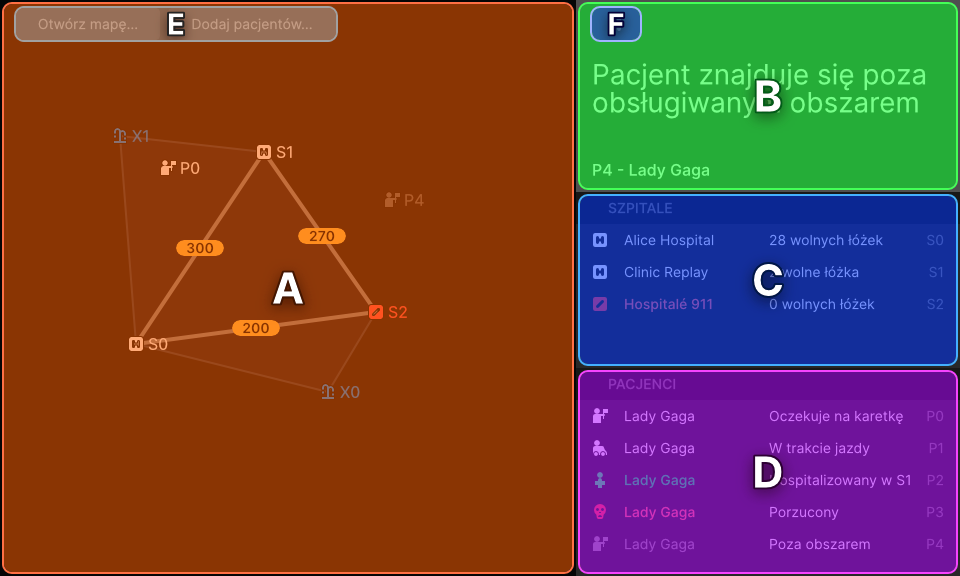
\includegraphics[scale=0.3]{images/areas.png}}

 \vspace{0.7cm}
 
\begin{itemize}
    \item A - mapa szpitali, obiektów i położeń pacjentów,
    \item B - sekcja informacyjna,
    \item C - lista szpitali,
    \item D - lista pacjentów,
    \item E - przyciski ładowania plików,
    \item F - przycisk kontroli symulacji ("Uruchom"/"Wstrzymaj")
\end{itemize}

\pagebreak
\subsubsection{Mapa}
Mapa przedstawia następujące informacje: \\

\centerline{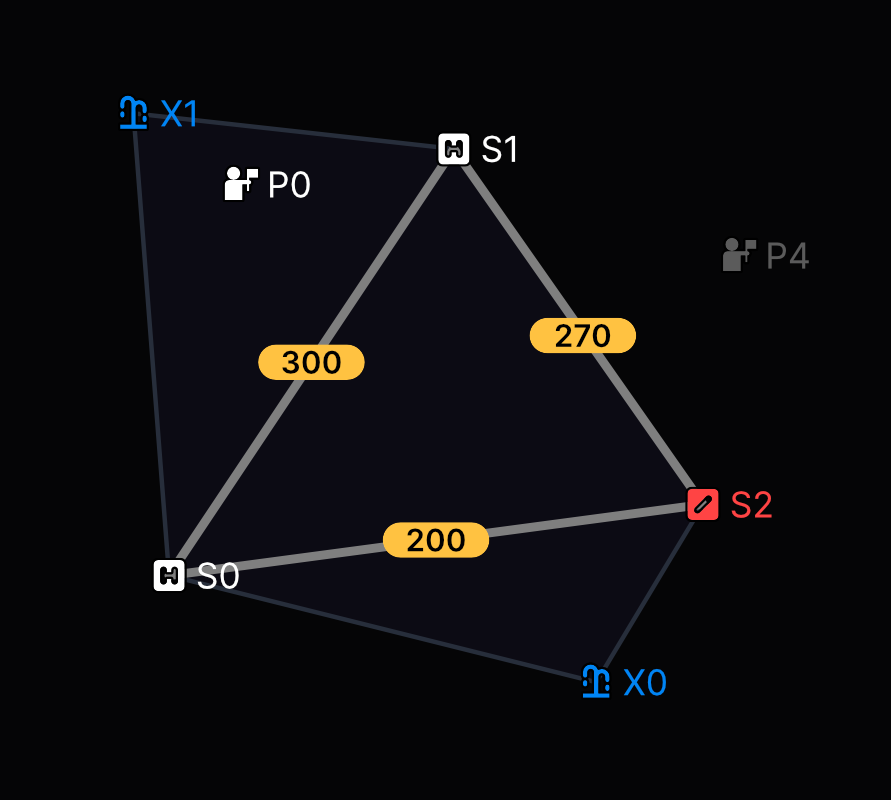
\includegraphics[scale=0.3]{images/map.png}}
 \vspace{0.7cm}
 
\begin{itemize}
    \item Szpitale (oznaczone literą S),
    \item Pacjenci (oznaczeni literą P),
    \item Inne obiekty (oznaczone literą X),
    \item Drogi między szpitalami (gruba szara linia),
    \item Obsługiwany region (ciemnoszara linia oraz wypełnienie),
    \item Długości odcinków dróg (żółte bloki)
\end{itemize}

Kolory niektórych obiektów przekazują dodatkowe informacje: czerwone szpitale nie mogą przyjmować więcej chorych, wyszarzeni pacjenci znajdują się poza obszarem. \\
Użytkownik może zmieniać widoczny na mapie region przesuwając widok (ruch myszki z naciśniętym prawym przyciskiem) lub zwiększając i zmniejszając widoczny obszar (Ctrl+kółko w górę, Ctrl+kółko w dół).

\subsection{Scenariusz działania}

\begin{enumerate}
    \centerline{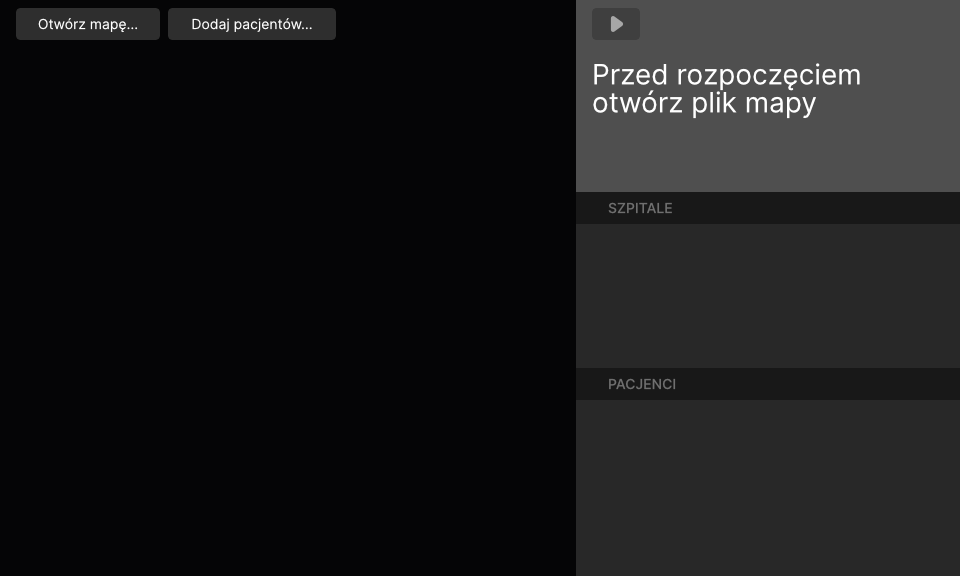
\includegraphics[scale=0.3]{images/state nomap.png}}
     \vspace{0.3cm}
    
    \item Dostarczenie pliku mapy oraz pacjentów. \\
          Program nie może rozpocząć symulacji bez obecności odpowiednich danych. \\
          Użytkownik musi wprowadzić do systemu:
          \begin{itemize}
              \item Plik mapy przez wciśnięcie przycisku "Otwórz mapę..." i wybranie odpowiedniego pliku,
              \item Dane pacjentów przez wciśnięcie przycisku "Dodaj pacjentów..." i wybranie odpowiedniego pliku,
                    bądź kliknięcie lewym przyciskiem myszy na mapie, powodując dodanie pacjenta w punkcie pod wskaźnikiem.
          \end{itemize}
          W przypadku, gdy wybrany plik wejściowy (mapy bądź pacjentów) jest niepoprawnie sformatowany,
          program wyświetli odpowiedni komunikat w sekcji informacyjnej:
          \begin{itemize}
              \item \emph{Niepoprawny plik mapy} - podany plik mapy jest niepoprawnie sformatowany bądź zawiera błędy.
              \item \emph{Niepoprawny plik pacjentów} - podany plik danych pacjentów jest niepoprawnie sformatowany bądź zawiera błędy.
          \end{itemize}
         
    \centerline{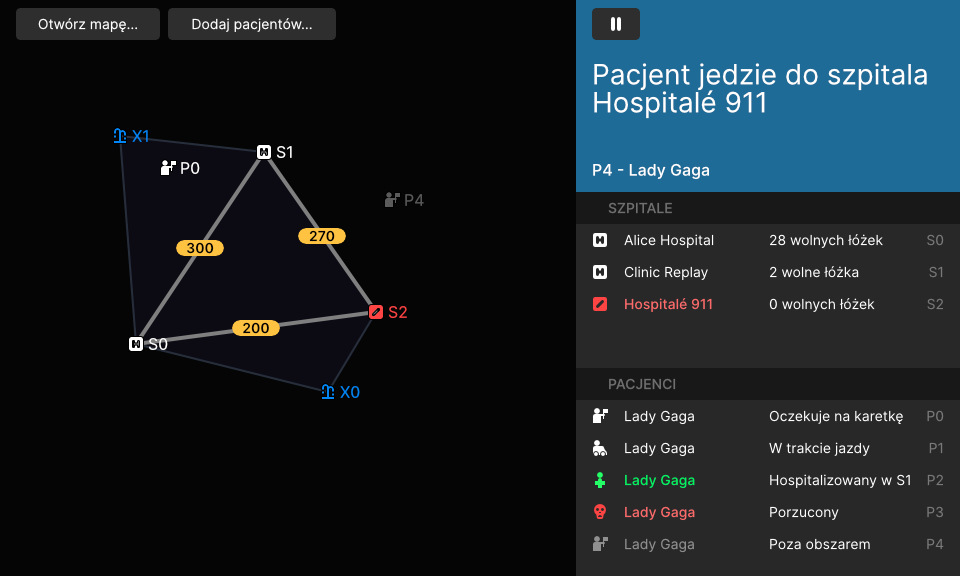
\includegraphics[scale=0.3]{images/state riding.png}}
    
    \item Rozpoczęcie symulacji. \\
          Jeśli wprowadzone dane były poprawne oraz kompletne, użytkownik może rozpocząć symulację przy użyciu przycisku "Uruchom". W trakcie trwania, ponowne wciśnięcie przycisku powoduje wstrzymanie działania algorytmu. \\
          Algorytm w trakcie trwania będzie przedstawiał kolejne stany działania zarówno na mapie, jak i w sekcji informacyjnej:
          \begin{itemize}
              \item \emph{Pacjent jedzie do szpitala X}
              \item \emph{W szpitalu X brakuje łóżek}
              \item \emph{Pacjent został przyjęty w X}
              \item \emph{Pacjent znajduje się poza obsługiwanym obszarem}
              \item \emph{Pacjent został porzucony}
          \end{itemize}
\end{enumerate}
\section{Testowanie}
Do testów jednostkowych wykorzystamy narzędzie JUnit 5, natomiast GUI będziemy sprawdzać w trakcie pisania programu.
\end{document}
